\chapter{RESULTS AND DISCUSSIONS}
\thispagestyle{empty}
\onehalfspacing
\pagestyle{fancy}
\fancyhf{}
\fancyhead[LE,RO]{\textit{\footnotesize \thepage}}
\fancyhead[RE,LO]{\textit{\footnotesize Avenue - Online Event Management System}}
%\fancyfoot[LE,LO]{\textit{\footnotesize Department of CSE}}
\fancyfoot[LE,RO]{\textit{\footnotesize Department of CSE}}
 
\renewcommand{\headrulewidth}{2pt}
\renewcommand{\footrulewidth}{1pt}
\section{ Results   }
\subsection{Home Page}
This is the first interface for the Avenue event management system. This interface can be
accessed by all the system users and has information about what has to be done to access
the different system functionalities
\begin{figure}[h]
	\centering
	\includegraphics[scale=0.11]{HomePage1.png}
	\includegraphics[scale=0.11]{HomePage2.png}
	\caption{Home Page}
	\label{Home Page}
\end{figure}
\subsection{Client Login/Signup Page}
The client must login into his account for booking any events. If he does'nt have an account, he must create one by signing up.
\begin{figure}[H]
	\centering
	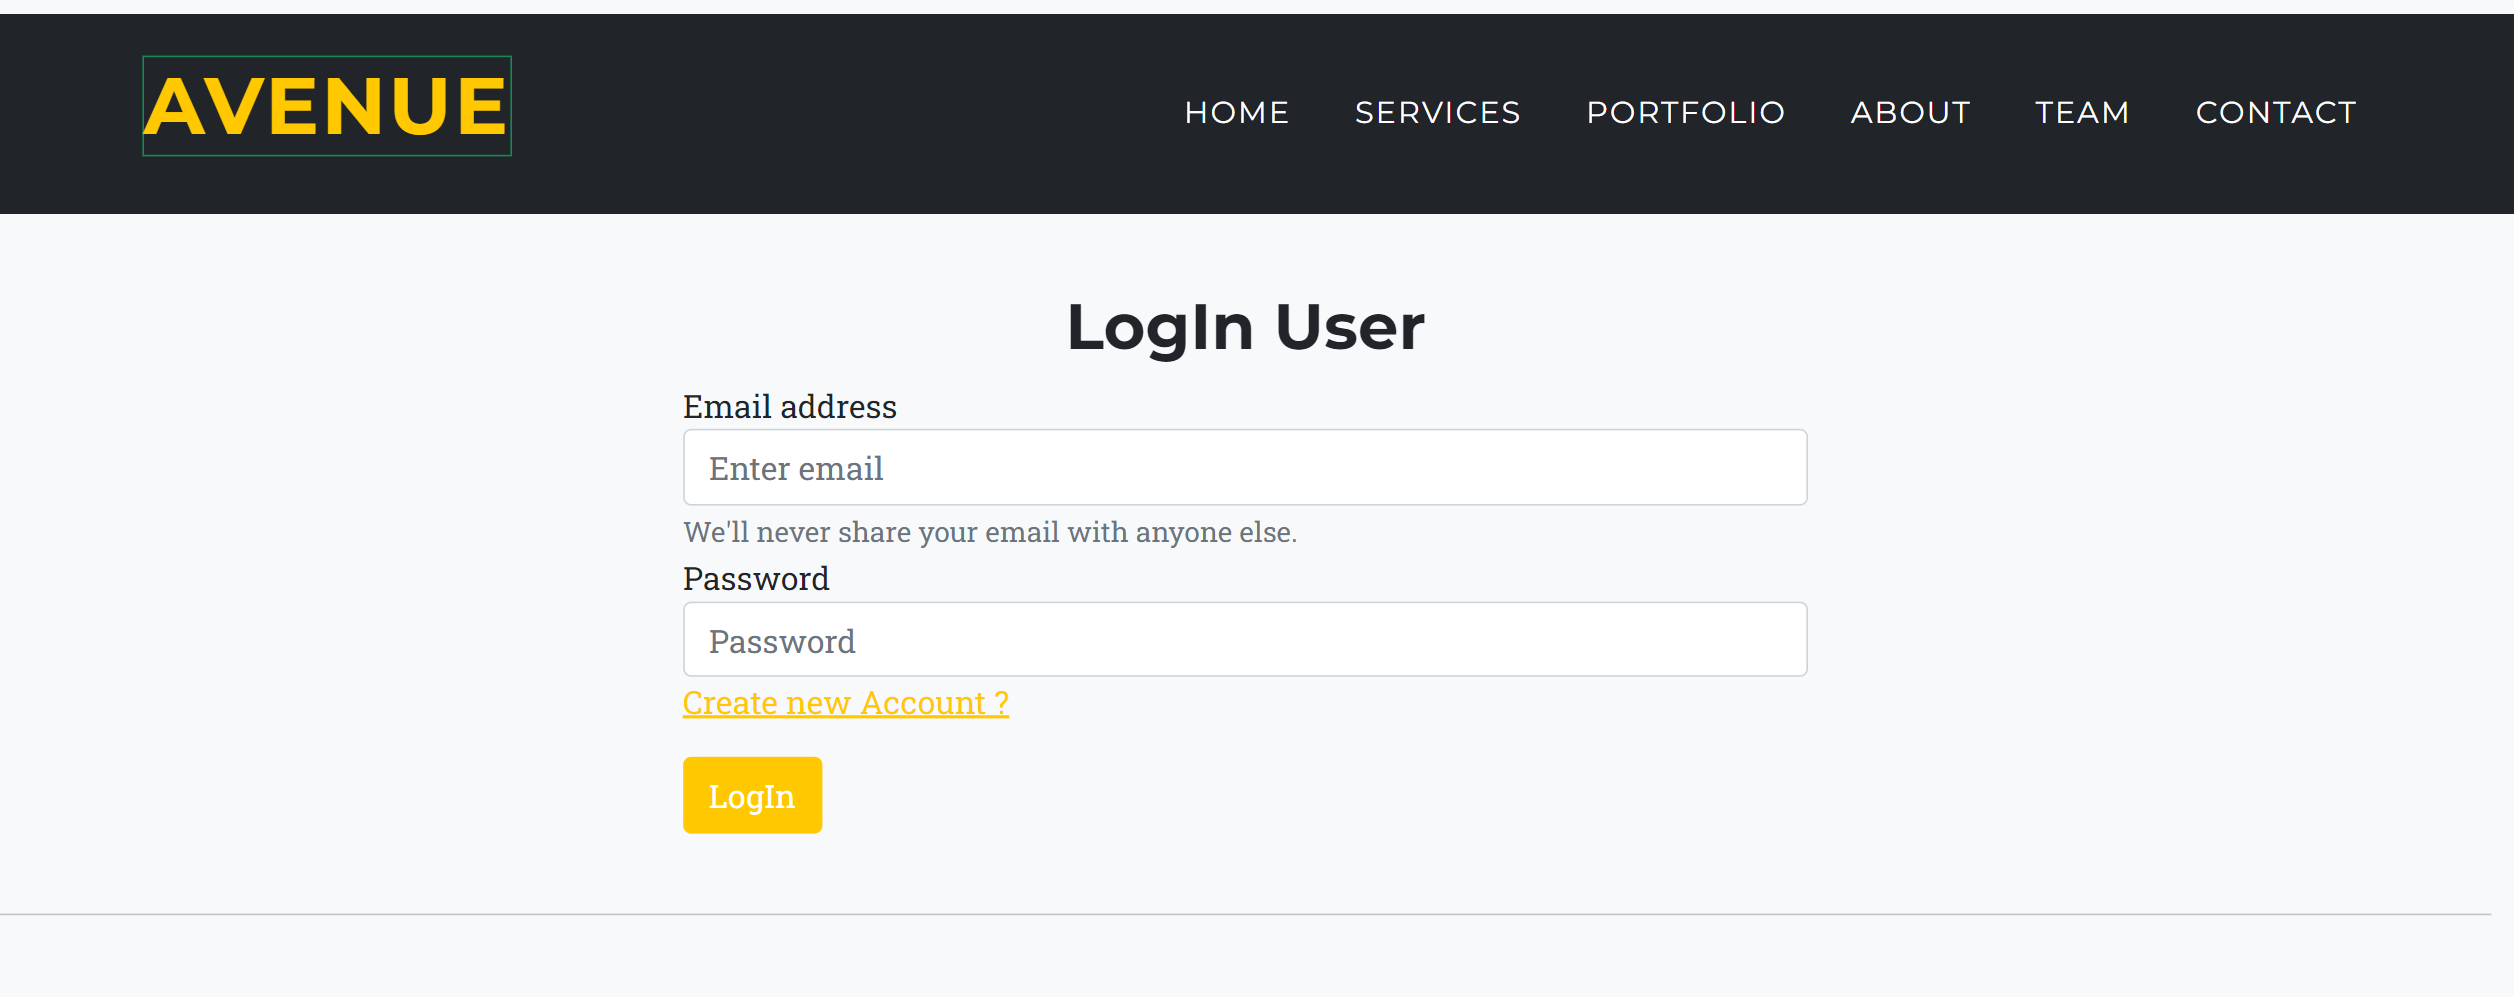
\includegraphics[scale=0.2]{login.png}\newline\newline
	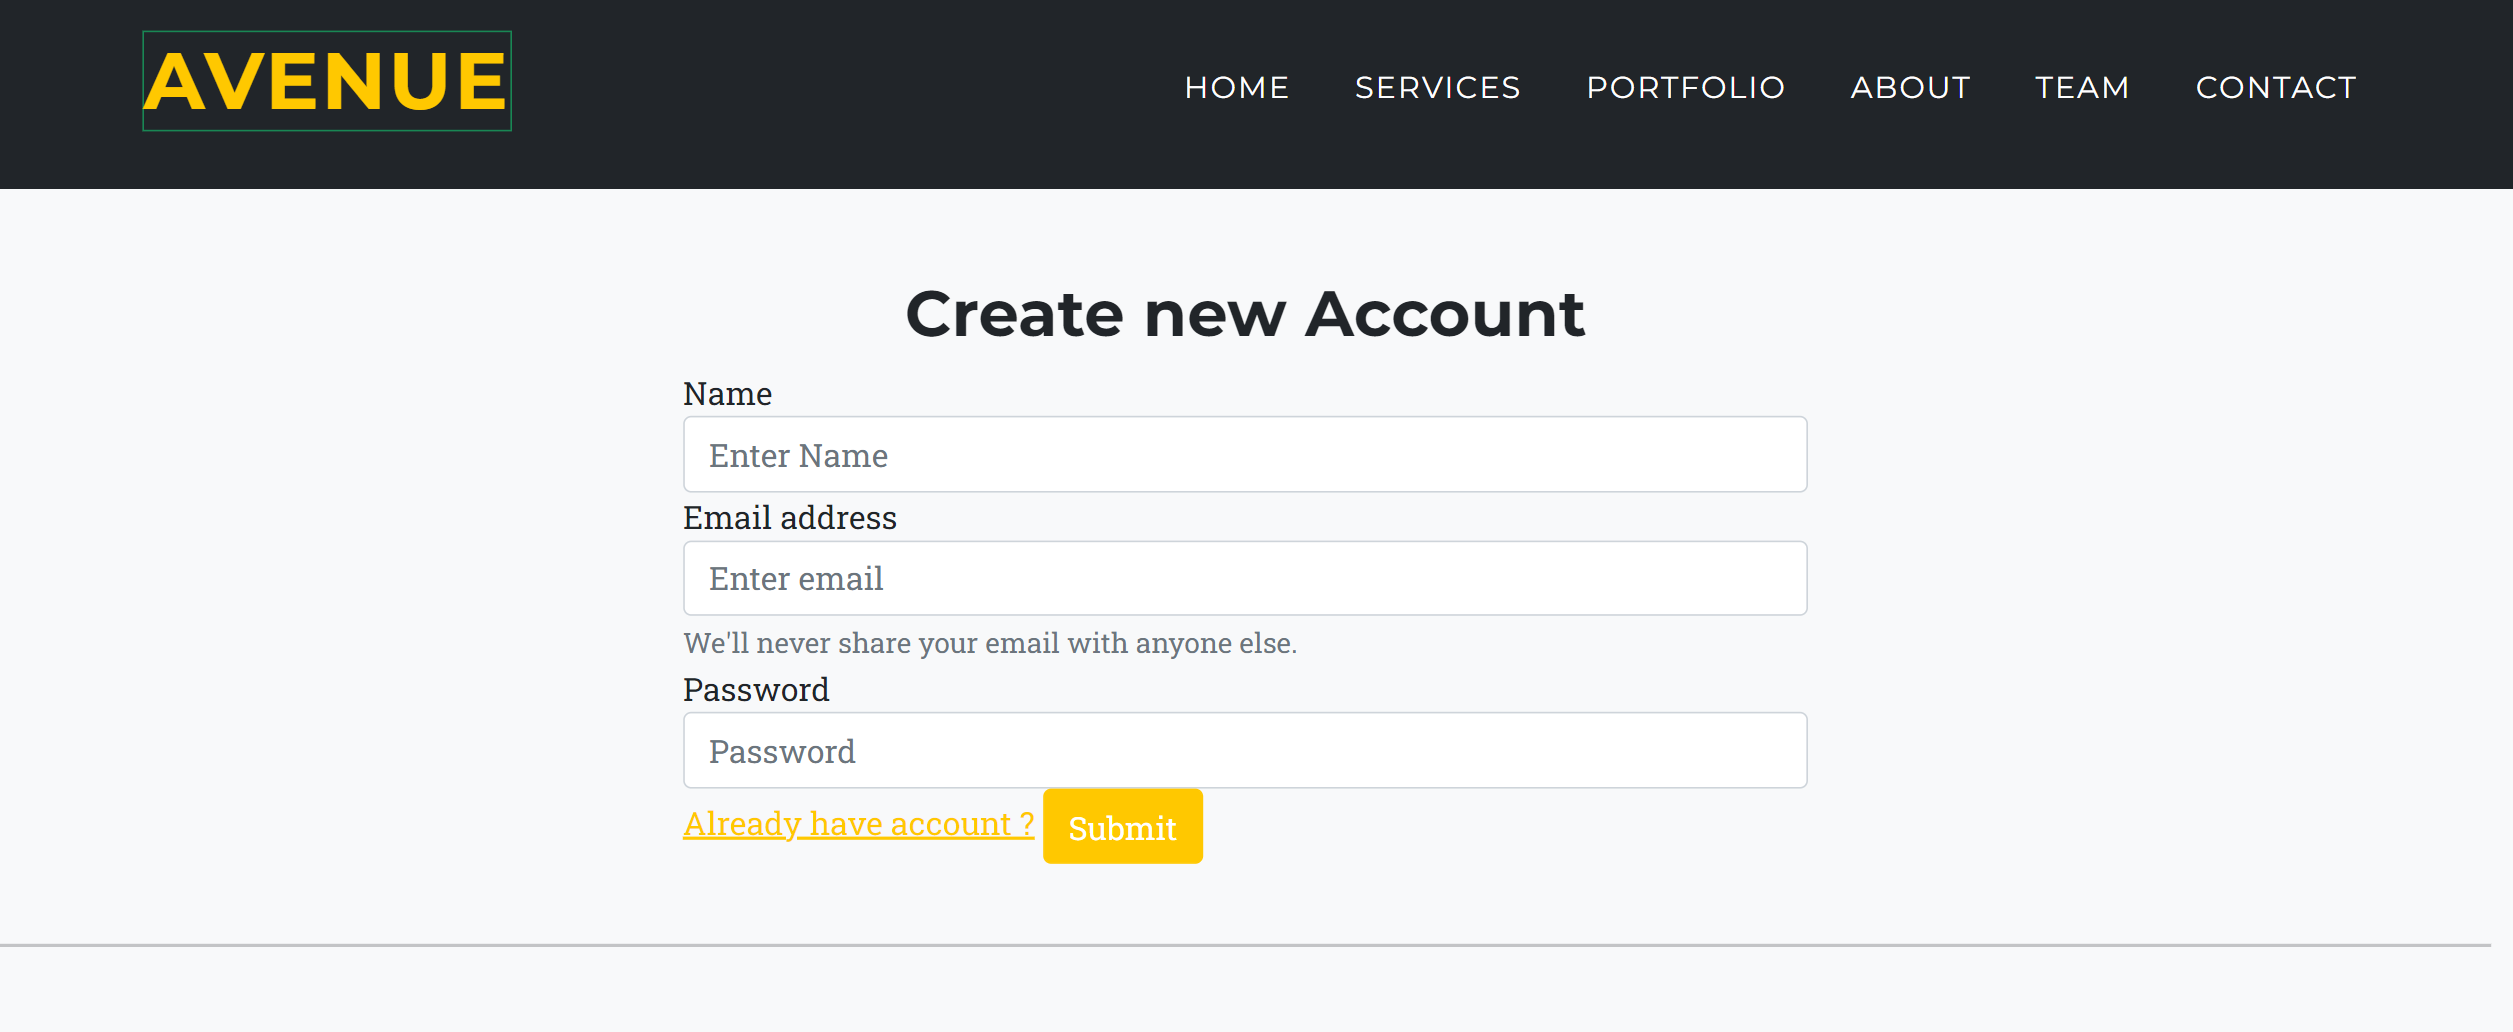
\includegraphics[scale=0.2]{signup.png}
	\caption{Login/Signup Page}
	\label{Login/Signup Page}
\end{figure}
\subsection{Client Booking Page}
The client will login after signing up and make a booking through this page as indicated
in the figure below. 
\begin{figure}[H]
	\centering
	\includegraphics[scale=0.17]{Contact.png}
	\caption{Booking Page}
	\label{Booking Page}
\end{figure}
\subsection{Event Planners Login and Account}
Event planners can login to their account where he can view his events and chat with his clients. He can also edit his profile details int the member account page.
\begin{figure}[H]
	\centering
	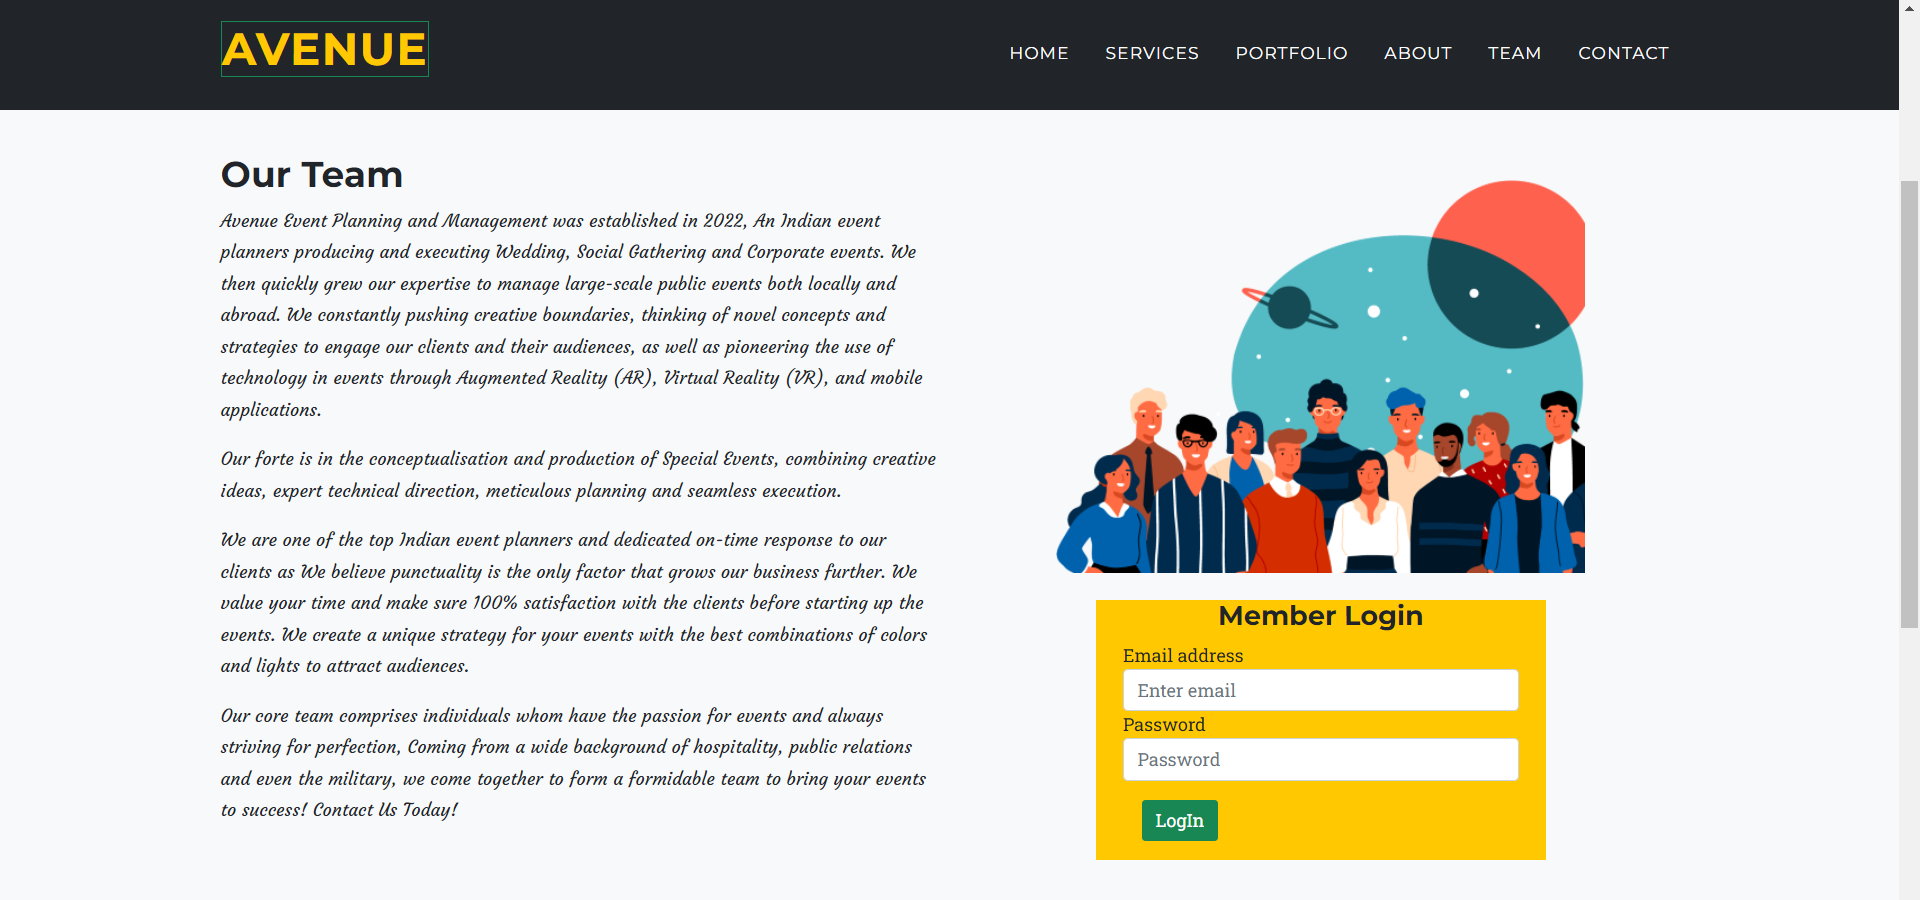
\includegraphics[scale=0.33]{memberlogin.png}
\end{figure}
\begin{figure}[H]
	\centering
	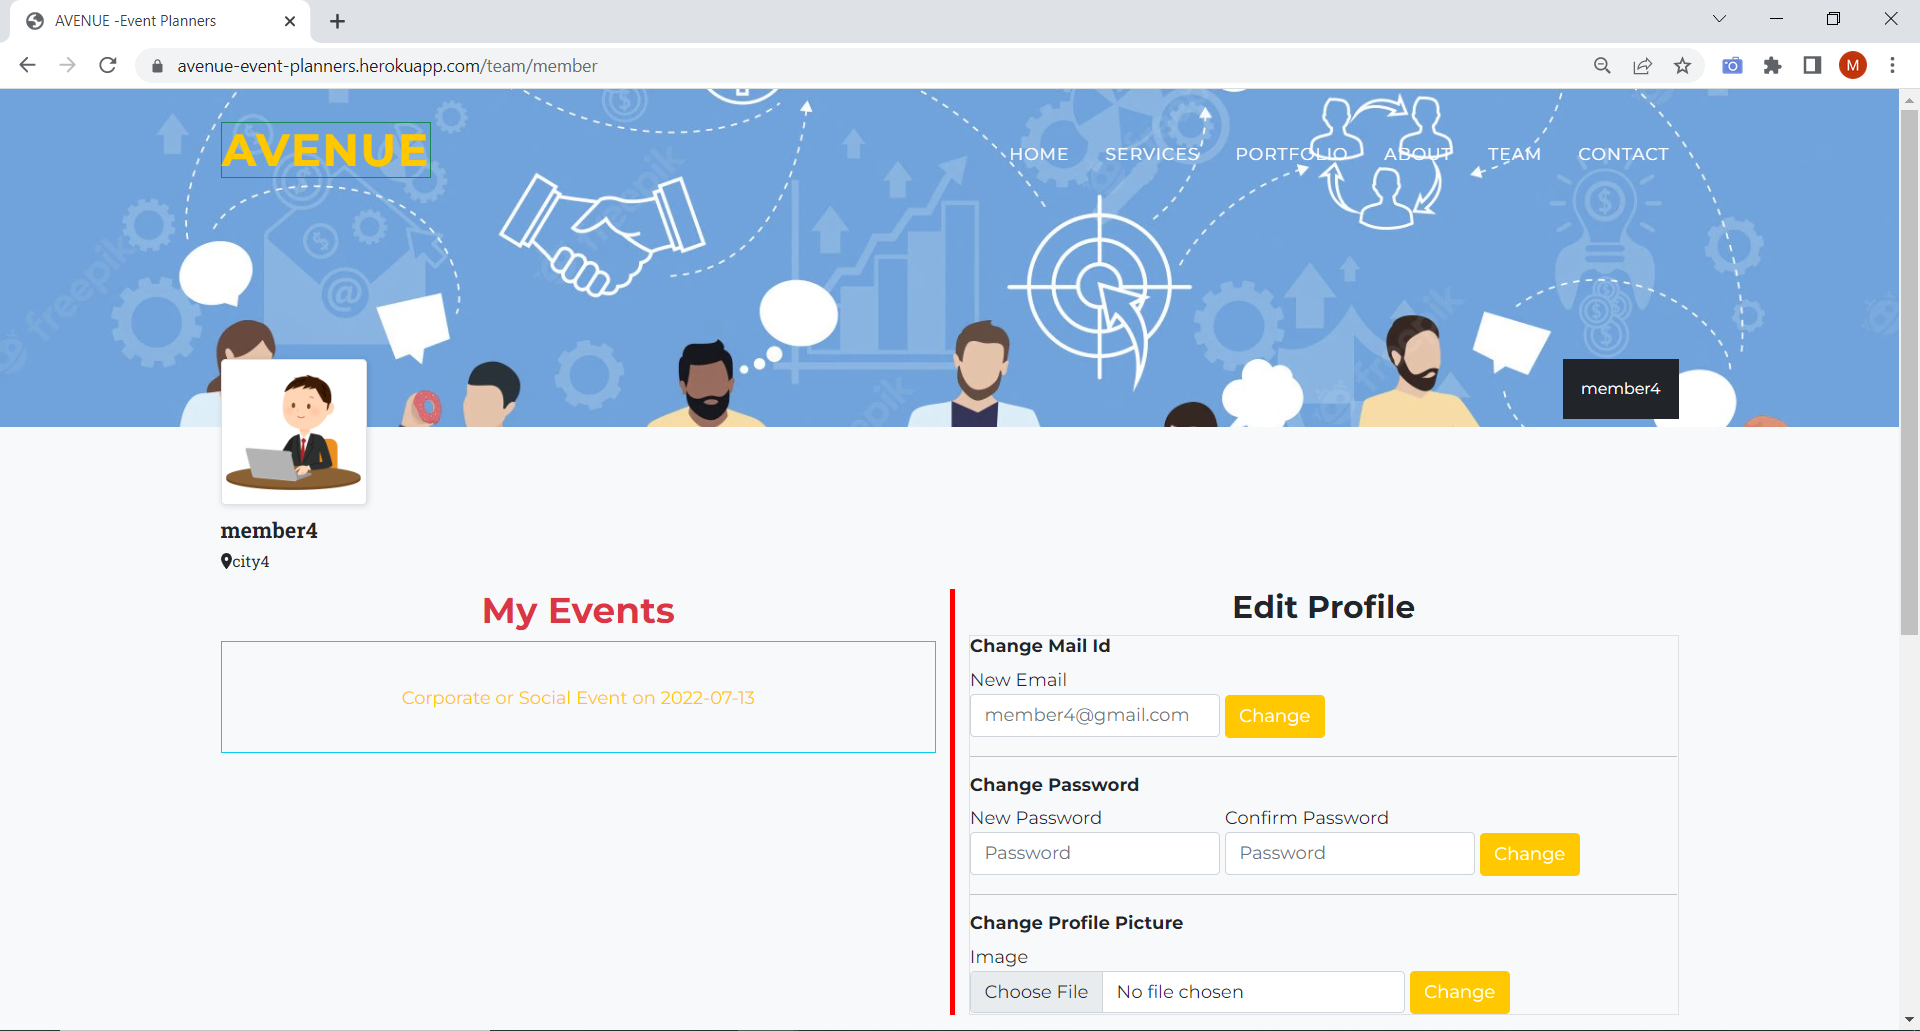
\includegraphics[scale=0.35]{memberaccount.png} \\
	\caption{Event Planners Login and Account Pages}
	\label{Event Planners Login and Account Pages}
\end{figure}
\subsection{Admin Login Interface}
Admin Login page is available in ' /admin ' route ,i.e, "BASE-URL/admin".Admin login details are matched with the login credentials already saved in the database.
\begin{figure}[H]
	\centering
	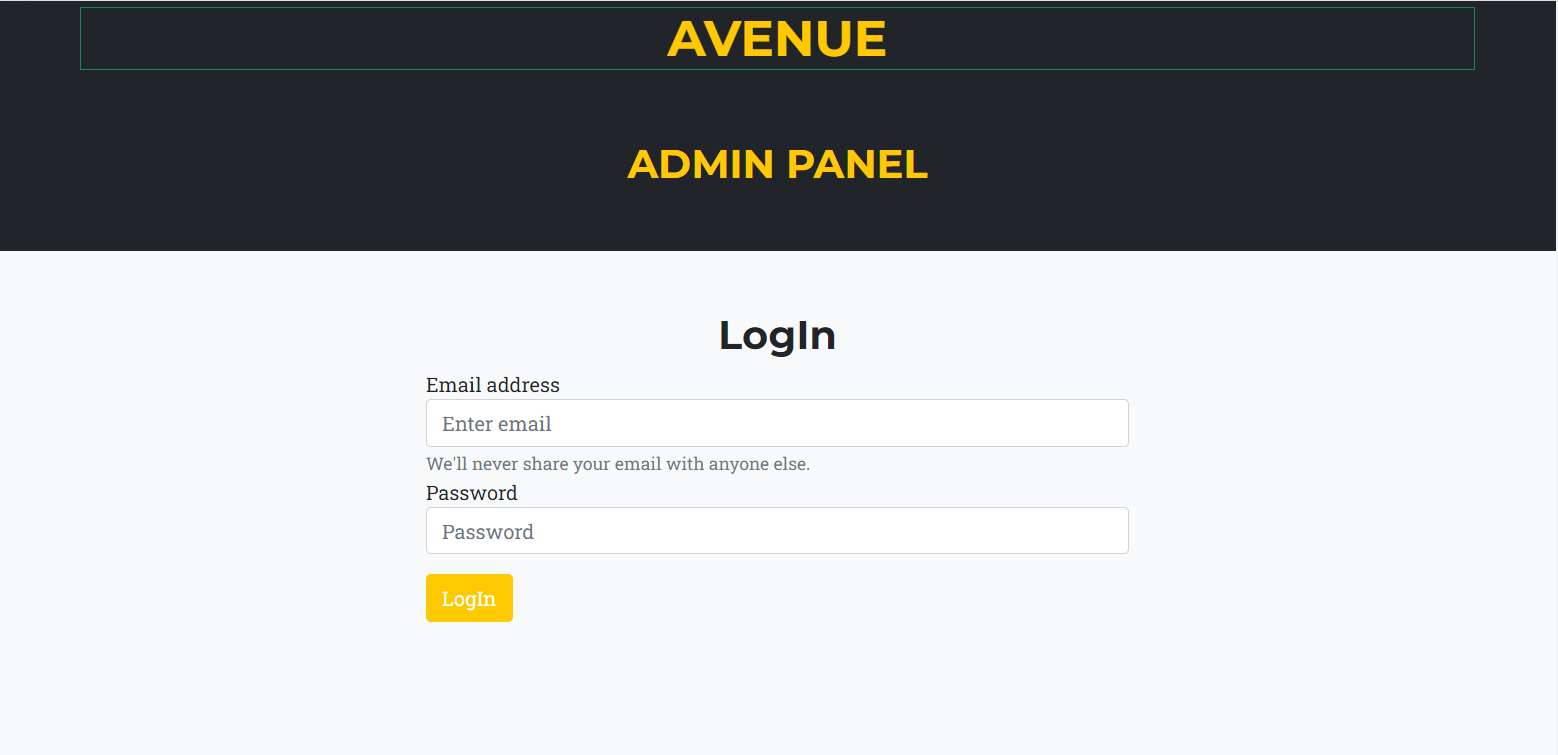
\includegraphics[scale=0.25]{adminlogin.png}
	\caption{Admin Login Page}
	\label{Admin Login Page}
\end{figure}
\subsection{Admin Panel Interface}
When the Username and Password is correct and the user privilege level is
Administrator, the user is then directed to the admin main switch board as indicated
below. 
\begin{figure}[H]
	\centering
	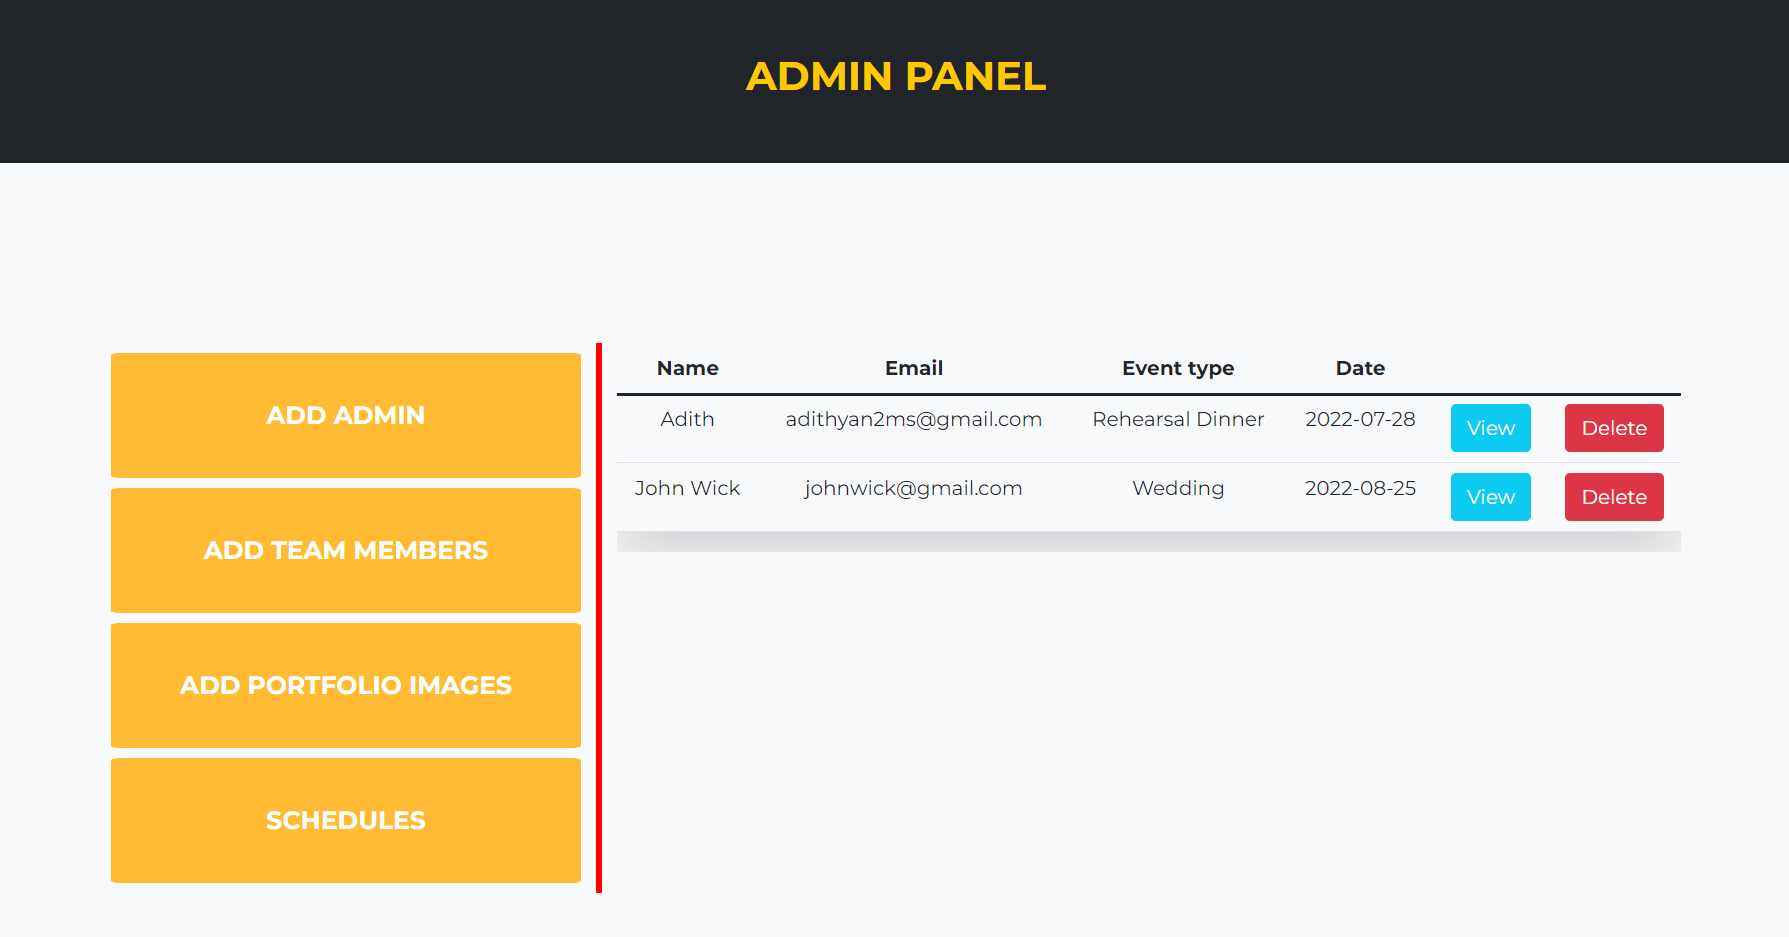
\includegraphics[scale=0.25]{adminhome.png}
	\caption{Admin Panel}
	\label{Admin Panel}
\end{figure}
\subsection{Admin Handling Requested Events}
Admin views all the event requests and accepts or rejects them based on certain circumtances like unavailability of members ,frank details etc.He also sets the event handling team before accepting the event.
\begin{figure}[H]
	\centering
	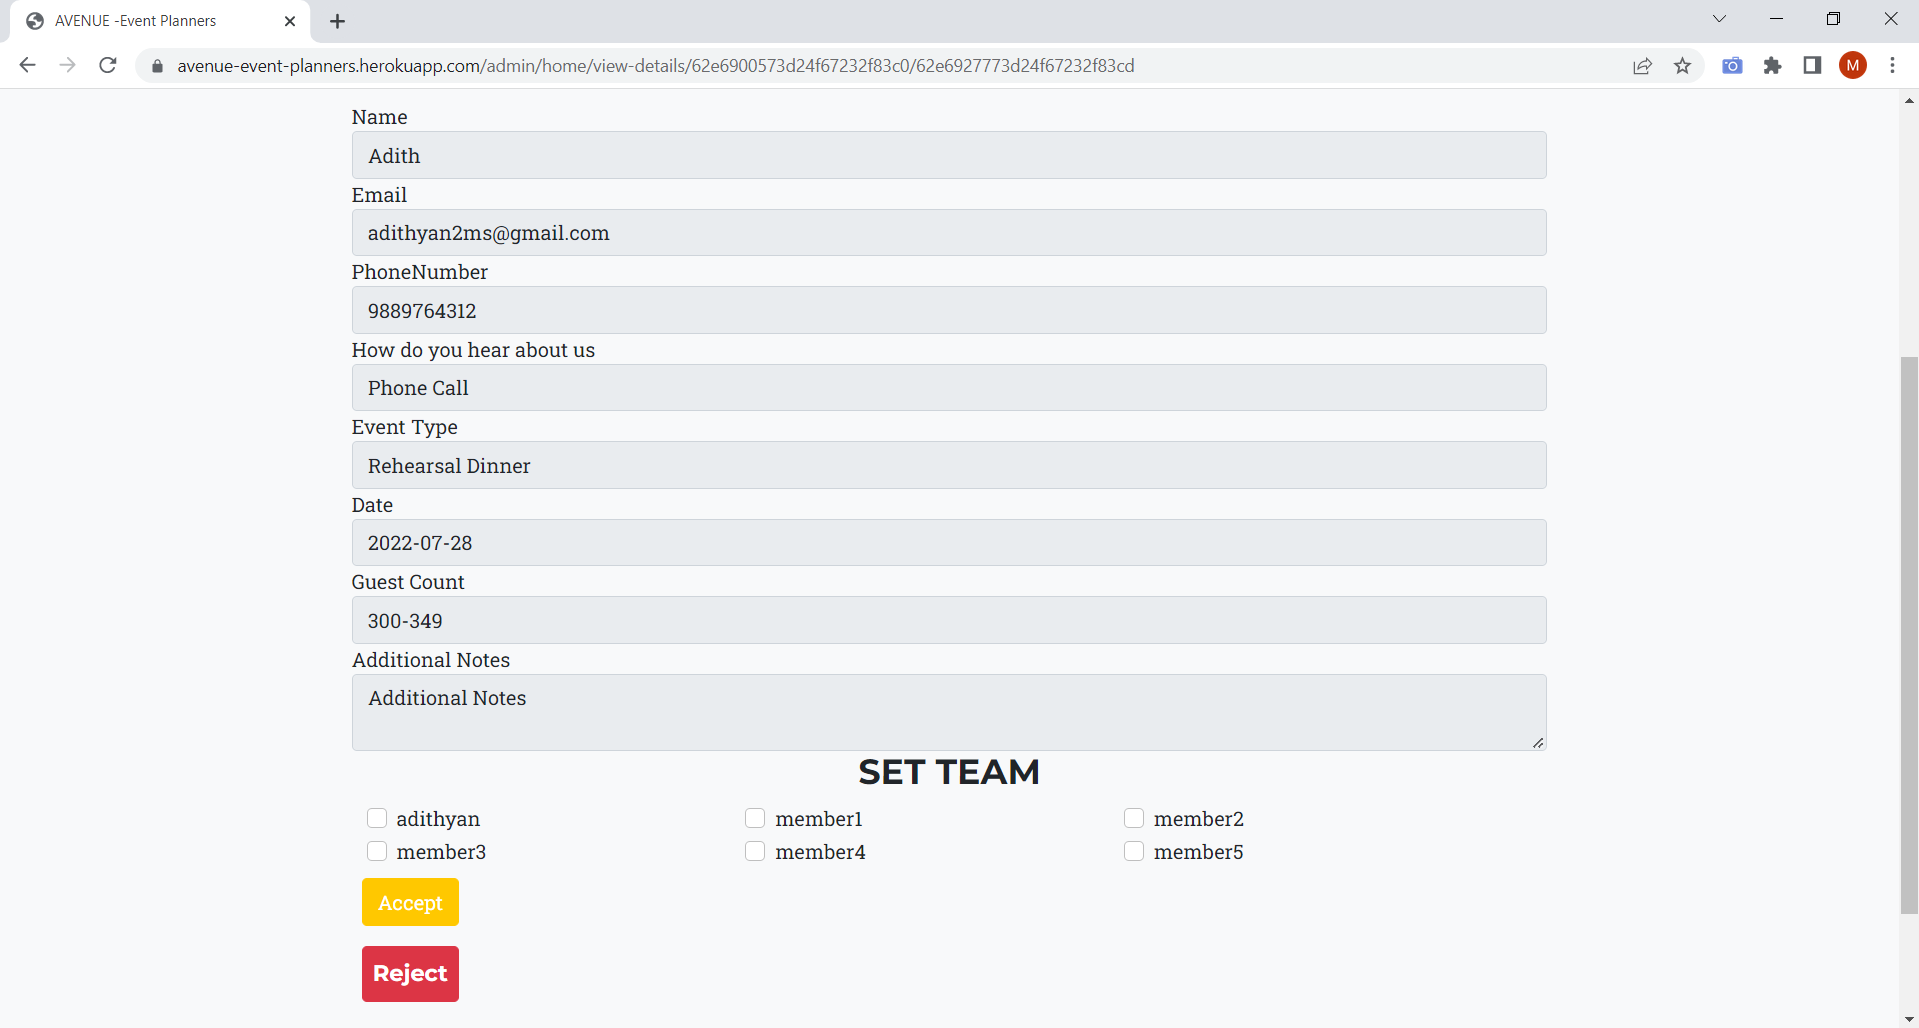
\includegraphics[scale=0.35]{adminview.png}
	\caption{Admin handling event request}
	\label{Admin handling event request}
\end{figure}
\subsection{Scheduled Events}
Events accepted by the admin are shown here containing the event details and the team members.
\begin{figure}[H]
	\centering
	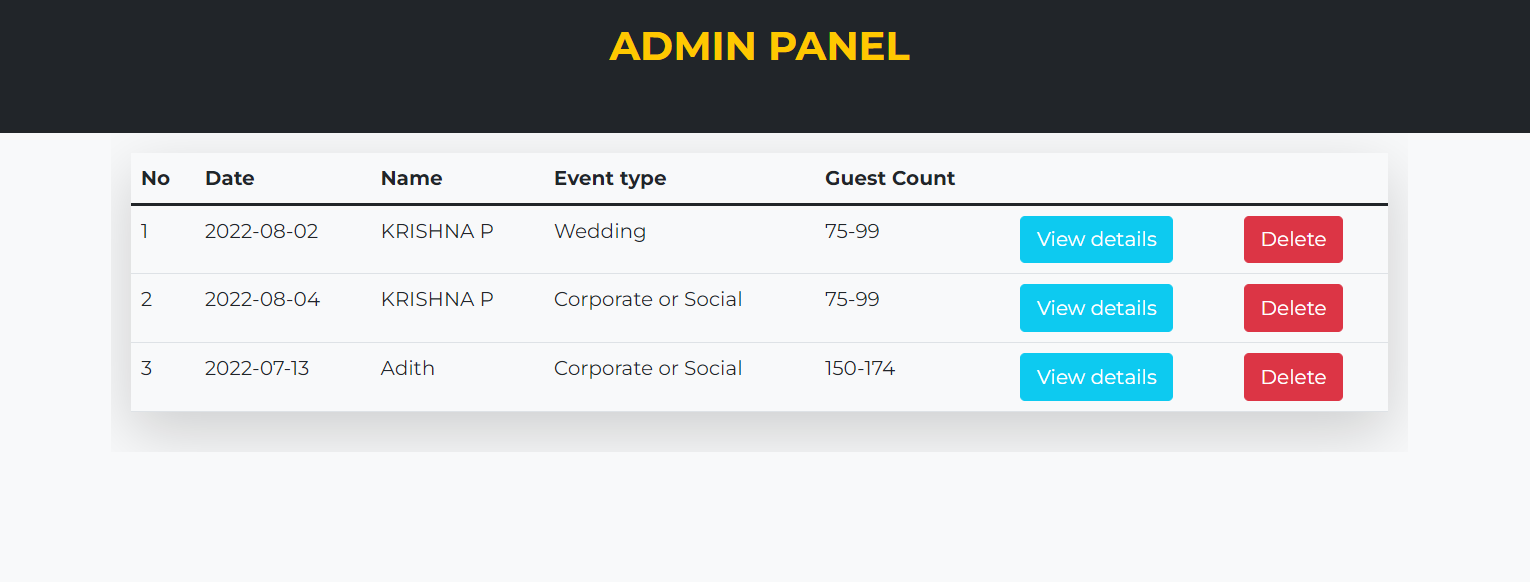
\includegraphics[scale=0.35]{scheduledevents.png}
	\caption{Scheduled Event Page}
	\label{Scheduled Event Page}
\end{figure}
\subsection{Adding Event Planners}
Admin adds new event planners details. After adding the details the login creditionals for the member's account are mailed to the planner's mailid.
\begin{figure}[H]
	\centering
	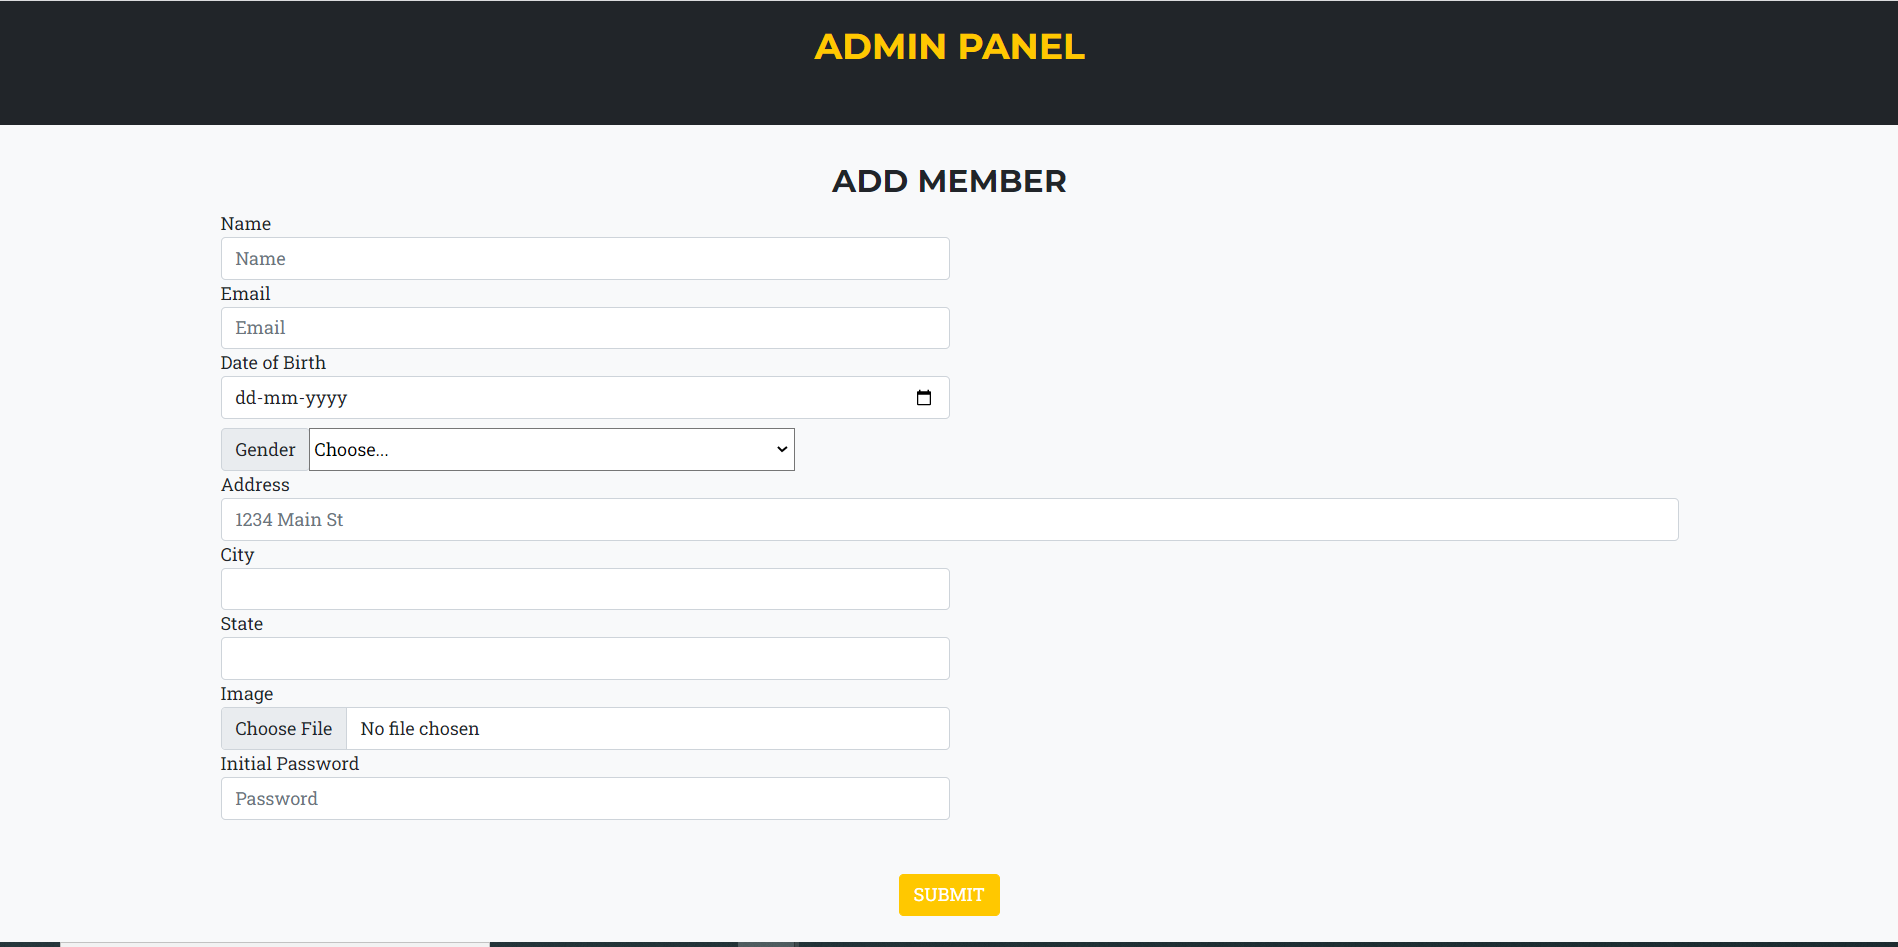
\includegraphics[scale=0.35]{addmember.png}
	\caption{Adding Members Page}
	\label{Adding Members Page}
\end{figure}
\subsection{Adding Portfolio Images}
Portfolio Images for the website added by the admins so that new event images can be updated occasionally.
\begin{figure}[H]
	\centering
	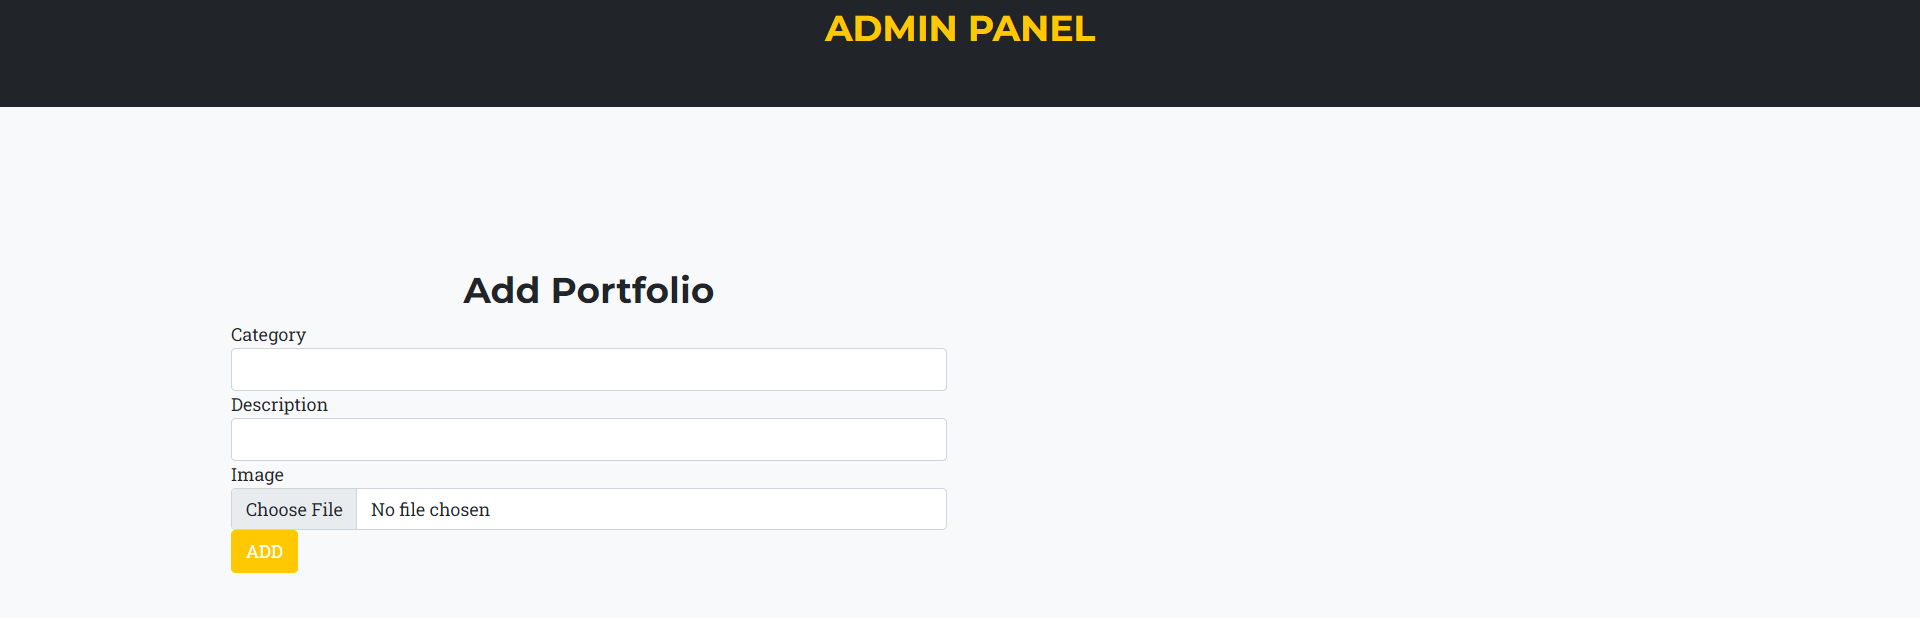
\includegraphics[scale=0.35]{addportfolio.png}
	\caption{Add Portfolio images Page}
	\label{Add Portfolio images Page}
\end{figure}
\subsection{Chat Page}
Once the event has been scheduled the client can chat with the event planners using the chat interface.
\begin{figure}[H]
	\centering
	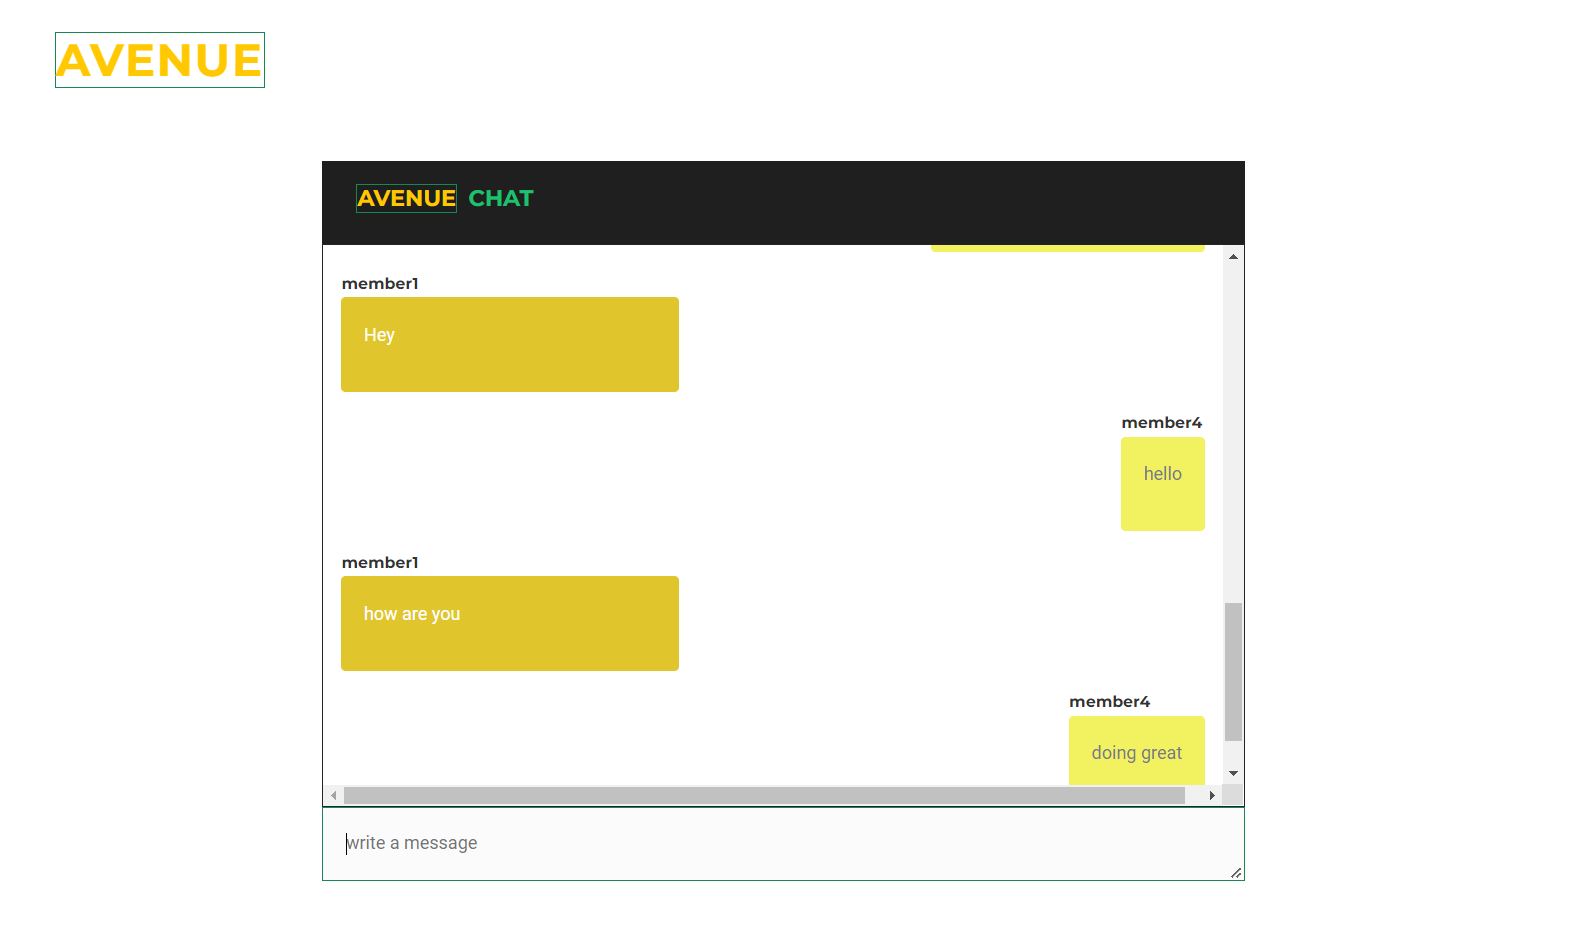
\includegraphics[scale=0.4]{chatpage.png}
	\caption{Chat Page}
	\label{Chat Page}
\end{figure}

\section{Discussion of Results   }
The main objective of the research project was to design and develop an online event management system. The project aim was automating the processes of booking and handling the events at Avenue Event Managem
through the Design and Development of an online event management system.
\newline
A number of steps are summarized in terms of the four specific objectives. The achievement of these specific objectives is explained
below; 
 \newline
The first specific objective was to review the current event managements system. This
was done in chapter two where a number of literatures relating to the research problem
were reviewed which helped in identifying the gaps in the related work that was already
done by other researchers \newline
The requirements of the proposed system i.e. user and system requirements were
collected and analyzed using different methodologies as discussed in chapter three. The proposed system requirements and the system designs are also explained in the same chapter.
\newline
The third specific objective was to develop the online Event Management System. The
System was developed basing on the designs presented in chapter 3, Software
tools like NodeJS, MongoDB, HTML ,CSS and JavaScript were used in the development
process. \newline
All the activities mentioned above were done with the main aim of achieving what was
proposed.












